\documentclass[10pt,twocolumn]{article}
\usepackage{graphicx}
\usepackage{amsmath}
\usepackage{booktabs}
\usepackage[margin=1in]{geometry}
\usepackage{authblk}
\usepackage{hyperref}
\usepackage{float}
\usepackage{caption}

% Handle figures in two-column layout better
\usepackage{stfloats}

% Title formatting
\title{\Large \textbf{Investigating Neuron Responses to Stimulus Orientation in Static and Drifting Gratings}}

\author{
  Umut Tuna Akgul, Utku Bahcivanoglu, Tommaso Ferracina, George Morris, Tebe Nigrelli
}


\begin{document}

\maketitle

\begin{abstract}
In this study, we analyze ecephys data from the Allen Brain Observatory to investigate how neural units in the mouse visual cortex respond to static and drifting gratings stimuli. Our aim is to identify brain regions and specific neurons that have a significant role in encoding stimulus orientation. We group neural firing rate across multiple trials and conditions to simplify the search. By selecting the most informative neurons based on their response, we construct a decoder capable of predicting stimulus orientation from neural activity.
\end{abstract}

\section{Introduction}

Understanding how the brain encodes visual information, particularly the perception of orientation in the visual cortex, is a central goal in neuroscience. Orientation selectivity—the tendency of neurons to respond preferentially to visual stimuli of a particular orientation—is a fundamental feature of early visual processing. However, understanding the dynamics of neuron excitation in the brain is challenging due to the intrinsic complexity of inter-neuron connectivity. This investigation uses neuron firing rate statistics to differentiate cross-region and cross-stimuli behavior, shedding light on the distinction between different static grating orientations. We also uncover the relationship between neurons in different cortical regions and propose a simple model to understand 'superstar' neurons and regions.

\section{Data Processing}

We started our investigation by searching the \textit{AllenSDK} dataset for a session containing units from different brain regions. We finally chose study \textit{750332458} for its balanced distribution of units, especially those related to the visual cortex (VIS). \textit{See Appendix A for regional distribution.}

The dataset consists of time-aligned responses of neuronal units to stimuli. Although both stimuli and responses are characterized by multiple features, for the purpose of our investigation we focus our observations by grouping the responses only by stimulus orientation, and focusing our statistical study on the mean firing rate of each unit, for fixed stimulus orientation.

\section{Exploratory Data Analysis}

Our investigation focuses on the relation between unit activations and the orientation of different grating stimuli.

\subsection{Decoding static vs drifting}

We explored how spike count and variability (across presentations) differed between static and drifting gratings in the visual cortex (VISam). We discovered that the spike count per presentation (spike mean) was generally much higher for the same units in drifting gratings than in static gratings. We tested these findings with a paired Wilcoxon signed-rank test (alpha=0.05) which revealed a significant p-value (0.000) allowing us to reject the null hypothesis that units fire equally frequently for static and drifting gratings. We then performed the same analysis on spike Coefficient of Variation (CV = std/mean) which revealed the reverse, units had greater variability when presented with static gratings (p-value 0.000). \textit{See Figures \ref{fig:spike_mean} and \ref{fig:spike_cv} in Appendix A for comparisons of spike mean and coefficient of variation between static and drifting gratings.}

We then built two Random Forest classifiers with 5-fold cross validation using just spike\_mean and spike\_CV respectively. Model 1 using spike\_mean attained an accuracy of 1.000 $\pm$ 0.000 and model 2 using spike\_CV attained 0.933 $\pm$ 0.033. Clearly it is easy to effectively decode whether the stimulus is static or drifting gratings from the simple measures such as spike count per presentation.

\subsection{Firing Rate Baseline}

We first observe how spiking rate varies between regions: in general, we notice a linear relation between the log of the mean and the log of the standard deviation of the firing rates. Visually, it is clear that simply observing mean and standard deviation is not enough to characterize the brain region, though some qualitative differences can be identified. The firing rate statistics across brain regions are presented in Figure \ref{fig:firing_rate_stats} in Appendix A.

For convenience, we also include both the single plots, showing each region singularly in Figure \ref{fig:firing_rate_single} in Appendix A. It should be noted that since some regions contain little data, any conclusion is heavily subject to noise, thus should be considered unreliable.

\section{Selection of Neurons}

\subsection{Orientation Selectivity Analysis}
We quantified orientation selectivity of neurons in the visual cortex using the Orientation Selectivity Index (OSI), defined as:
\begin{equation}
OSI = \frac{R_{preferred} - R_{orthogonal}}{R_{preferred} + R_{orthogonal}}
\end{equation}
where $R_{preferred}$ represents the mean firing rate at the preferred orientation and $R_{orthogonal}$ represents the mean firing rate at the orthogonal orientation (90° offset from preferred). This analysis revealed a subset of neurons with pronounced orientation tuning (OSI > 0.5), which will provide good grounds for training a model.

\subsection{Statistical Validation of Orientation Tuning}
To statistically validate orientation tuning, we employed one-way ANOVA tests for each unit, comparing spike counts across different orientation presentations. The null hypothesis posited equal mean spike counts across all orientations, with the alternative hypothesis suggesting significant response differences to at least one orientation. This analysis identified a substantial population of neurons (p < 0.05) exhibiting statistically significant orientation tuning, confirming the presence of orientation-encoding properties within the dataset.

\subsection{Selection Criteria for Neurons}
We established the following criteria for neuron selection:
\begin{enumerate}
    \item High orientation selectivity $(OSI > 0.5)$
    \item Statistically significant orientation tuning $(\mathrm{ANOVA} \ p < 0.05)$
\end{enumerate}

\subsubsection{Static}

This approach yielded a population of 43 orientation-selective neurons distributed in the visual cortex, with notable concentrations in the VISal and VISl areas. The anatomical distribution of these neurons aligns with established literature on the hierarchical organization of orientation processing in the mouse brain.

Visualization of orientation tuning curves from representative neurons revealed diverse response profiles, including:
\begin{itemize}
    \item Narrowly tuned neurons with a strong response to one specific orientation
    \item Neurons with a broader reaction to a few concurrent orientations
\end{itemize}

These different tuning properties are likely beneficial to the encoding of orientation in the visual cortex, helping to discriminate between different orientations of visual stimuli. Tuning curves for static gratings can be found in Figure \ref{fig:static_tuning} in Appendix A.

\subsubsection{Drifting}

The same approach for drifting gratings was then employed with the same selection criteria. It revealed 81 orientation-selective neurons (almost double) many of which had higher OSI values between 0.8-1.0. Similarly, all were located in the visual cortex, predominantly in VISal, bar one which was in 'grey'.

The tuning curves were similarly conveying diverse response profiles with very strong responses to specific orientations. Though, the drifting tuning curves showed more peakedness around the preferred orientation, this is probably largely due to the fact that the difference between adjacent orientations is 45° instead of 30° and is not solely because the grating is drifting. These tuning curves are presented in Figure \ref{fig:drifting_tuning} in Appendix A.

Moreover, unlike Static here the orientations spanned a full 360° with the 45° increments giving 8 different orientations. A very interesting result was that orientations 180° apart both had very strong responses, where the gratings has the same orientation but is drifting in the opposite direction. Indeed it seems the units in general seemed to be more selective to orientation than direction. We wanted to test this by investigating DSI (Direction-sensitivity index).

\begin{equation}
DSI = \frac{R_{preferred} - R_{opposite}}{R_{preferred} + R_{opposite}}
\end{equation}

Using the same selection criteria above except using DSI > 0.5 instead only 8 neurons were left over supporting this hypothesis.

\section{Decoding Orientation from Neural Activity}

To assess whether the activity patterns of orientation-selective neurons could reliably predict stimulus orientation, we implemented a machine learning approach using the spike counts of selected neurons as features. The static dataset consisted of spike count responses to static grating stimuli presented at six distinct orientations (0°, 30°, 60°, 90°, 120°, and 150°). Whereas the drifting dataset the same but from 8 distinct orientations (0°, 45°, 90°, 135°, 180°, 225°, 270°, 315°, 360°) as direction is considered. The classification task involved predicting the stimulus orientation from the corresponding neural activity patterns.

\subsection{Data Preparation and Model Training}
We constructed a feature matrix where each row represented a stimulus presentation (indexed by stimulus\_condition\_id) and each column represented the spike count of an orientation-selective neuron. The target variable consisted of the corresponding orientation values. The dataset was stratified and split into training (70\%) and testing (30\%) sets to ensure proportional representation of all orientation classes. The static dataset consists of 20 presentations per orientation whereas the drifting dataset only consists of 5 presentations per orientation, a limitation to be considered.

Prior to model training, features were standardized using z-score normalization to account for differences in baseline firing rates across neurons. We evaluated three classification algorithms:

\begin{itemize}
    \item Random Forest Classifier
    \item Support Vector Machine (SVM) with linear kernel
    \item Multinomial Logistic Regression
\end{itemize}

\subsection{Classification performance}

\subsubsection{Results}

The following tables show the performance of our classifiers for static and drifting gratings respectively:

\begin{table}[ht]
\centering
\begin{tabular}{l c}
\hline
\textbf{Model} & \textbf{Accuracy} \\
\hline
Random Forest        & 0.8611 \\
SVM                  & 0.8333 \\
Logistic Regression  & 0.8889 \\
\hline
\end{tabular}
\caption{Classification accuracy for static gratings.}
\label{tab:static_performance}
\end{table}

Feature selection for static gratings is visualized in Figure \ref{fig:static_feature} in Appendix A. The confusion matrices for Random Forest, SVM, and Logistic Regression models for static gratings are presented in Figures \ref{fig:static_rf_cm} and \ref{fig:static_svm_logr_cm} in Appendix A.

\begin{table}[ht]
\centering
\begin{tabular}{l c}
\hline
\textbf{Model} & \textbf{Accuracy} \\
\hline
Random Forest        & 0.9167 \\
SVM                  & 1.0000 \\
Logistic Regression  & 1.0000 \\
\hline
\end{tabular}
\caption{Classification accuracy for drifting gratings.}
\label{tab:drifting_performance}
\end{table}

Feature selection for drifting gratings is visualized in Figure \ref{fig:drifting_feature} in Appendix A. The confusion matrices for Random Forest, SVM, and Logistic Regression models for drifting gratings are presented in Figures \ref{fig:drifting_rf_cm} and \ref{fig:drifting_svm_logr_cm} in Appendix A.

\subsubsection{Model conclusions}

Why did we get much better results for decoding drifting gratings? A number of factors. Firstly, we have more orientation-selective neurons available as features 81 vs 43. Secondly, more of these neurons have higher OSI values. However, it must be considered that the difference in orientation is 30° for static and 45° in drifting which might have an effect on decoding orientation. Another noteworthy comment is that our model is limited by the fact we only have 5 stimulus presentations for drifting and 20 for static.

\subsection{Cross condition analysis between static and drifting stimuli}

\subsubsection{Distribution of the OSI values}

At this point we wanted to dig deeper into the difference in OSI between static and drifting gratings by looking at the distribution of the OSI values. A comparison of tuning curves between static and drifting gratings is shown in Figure \ref{fig:tuning_comparison} in Appendix A.

Looking into the skewness and kurtosis:

Static Gratings:
\begin{itemize}
  \item Skewness : 2.258
  \item Kurtosis : 5.009
\end{itemize}

Drifting Gratings:
\begin{itemize}
  \item Skewness : 1.937
  \item Kurtosis : 3.397
\end{itemize}

We can draw a number of conclusions from the distribution of OSI values for units between the two stimuli.

\begin{enumerate}
    \item As we would expect the distribution is highly non-normal. Only a few neurons have a high OSI and are responsible for interpreting orientation.
    \item Drifting activates more neurons with high OSI overall.
    \item Static distribution illicits a higher kurtosis (5.009 > 3.397) indicating a narrower sharper peak and heavier tails than drifting. This suggests fewer relatively higher tuned neurons. This can probably be interpreted as the drifting nature of the grating is a kind of noise which triggers a greater response in neurons in general instead of a few concentrating on orientation only.
\end{enumerate}

Interestingly we see these results in the feature selection of our random forest models for static and drifting. For static fewer units make up a relatively much larger impact on the models decision than for drifting gratings. As for drifting many units have a high OSI value. 

\subsubsection{Distribution of orientation-selective neurons over regions}

The distribution of well-tuned neurons across brain regions is very similar given that there are twice as many well-tuned neurons for drifting as static, as shown in Figure \ref{fig:tuned_regions} in Appendix A. Only exceptions are that VISl seems to have greater relative importance for static stimuli whereas VISrl has greater relative importance for drifting. It would be interesting to see if this is the case in other sessions as well.

\subsubsection{Overlapping neurons for static and drifting}

We were also interested to see if it was the same units that were orientation-selective for both static and drifting gratings. We found that of the 43 units identified as significant for static gratings 29 were also significant for drifting gratings, well over half conveying it is largely the same units dealing with orientation in both cases as we might expect.

\section{Conclusions}

We can draw a number of conclusions from our analysis into decoding orientation from gratings stimulus. Principally, it is indeed possible to effectively decode the orientation of gratings from neural response using the spike count over presentations. It seems especially effective for drifting gratings where units have higher OSI values and are generally more orientation-selective. We also found however that of those orientation-selective neurons in static gratings they had a relatively much higher OSI score. This was conveyed by the static distribution of OSI values having higher kurtosis and was reflected in the feature importance of the model.

\section{Limitations and suggestions for further study}

There are a few limitations to our study. Largest of all is that there is a discrepancy in the angle of orientation between the static and drifting stimulus given to use in the AllenSDK dataset, 30° differences in static vs 45° in drifting. This is a large limitation on comparing our relative model performance between the two stimuli. However, it does not really limit our comparative analysis for OSI as this uses the preferred and orthogonal values for stimulus count which is the same for both. Nevertheless, it would be interesting in further study to have the same orientations for both and then to measure the difference in decoding performance.

Another big limitation is naturally that here we have only looked at one session of one mouse. Further research should perform the same procedure with other mice to see if the results are consistent.

Finally, another limitation lies in the nature of the stimulus gratings. Here we have focused on the orientation only. However, for static gratings the spatial frequencies and phases also varies while in drifting the temporal frequency varies. More stringent analysis should control these variables and keep the constant over presentations.

\newpage

\appendix

\section{Appendix A}

\begin{table}[h]
\centering
\begin{tabular}{lr}
\toprule
region & count \\
\midrule
grey   & 558 \\
VISal  &  71 \\
VISp   &  63 \\
VISam  &  60 \\
VISrl  &  44 \\
VISl   &  38 \\
VISpm  &  19 \\
CA1    &  16 \\
CA3    &  15 \\
DG     &   7 \\
\bottomrule
\end{tabular}
\caption{Distribution of units across brain regions.}
\label{tab:regions}
\end{table}

\begin{figure}[ht]
\centering
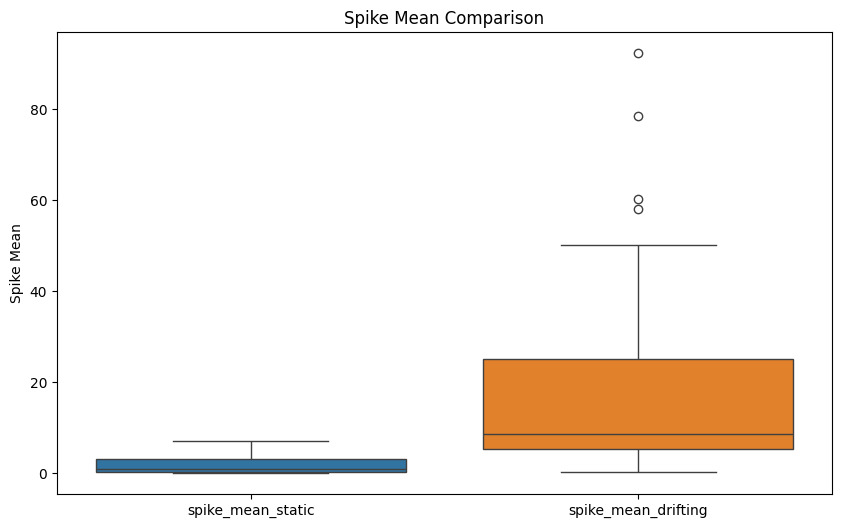
\includegraphics[width=0.85\linewidth]{report_images/spike_mean_comparison.png}
\caption{Spike mean: static and drifting}
\label{fig:spike_mean}
\end{figure}

\begin{figure}[ht]
\centering
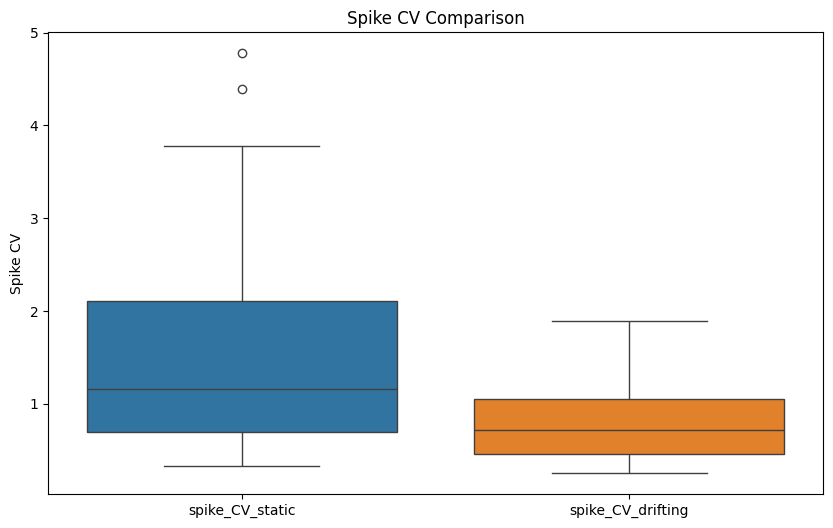
\includegraphics[width=0.85\linewidth]{report_images/spike_CV_comparison.png}
\caption{Spike CV: static and drifting.}
\label{fig:spike_cv}
\end{figure}

\begin{figure}[ht]
\centering
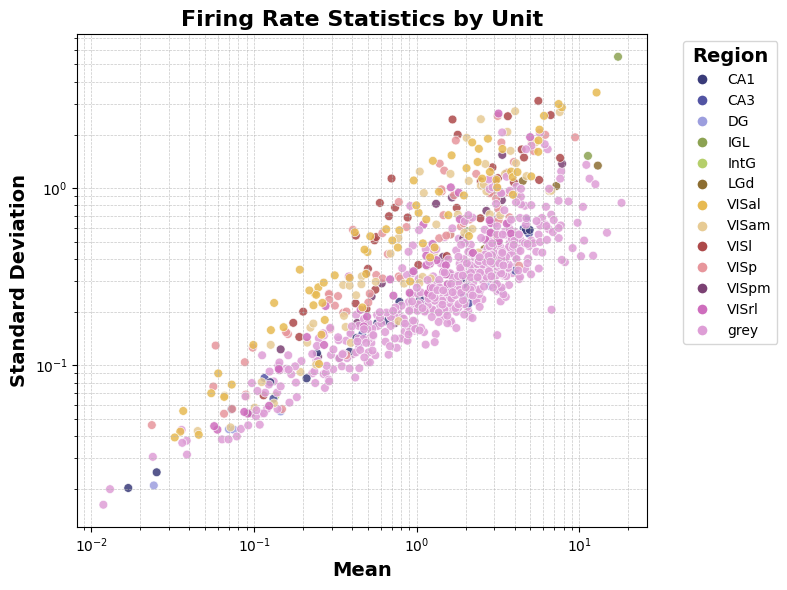
\includegraphics[width=\linewidth]{report_images/unit_firing_rate_statistics.png}
\caption{Firing rate statistics across brain regions.}
\label{fig:firing_rate_stats}
\end{figure}

\begin{figure}[ht]
\centering
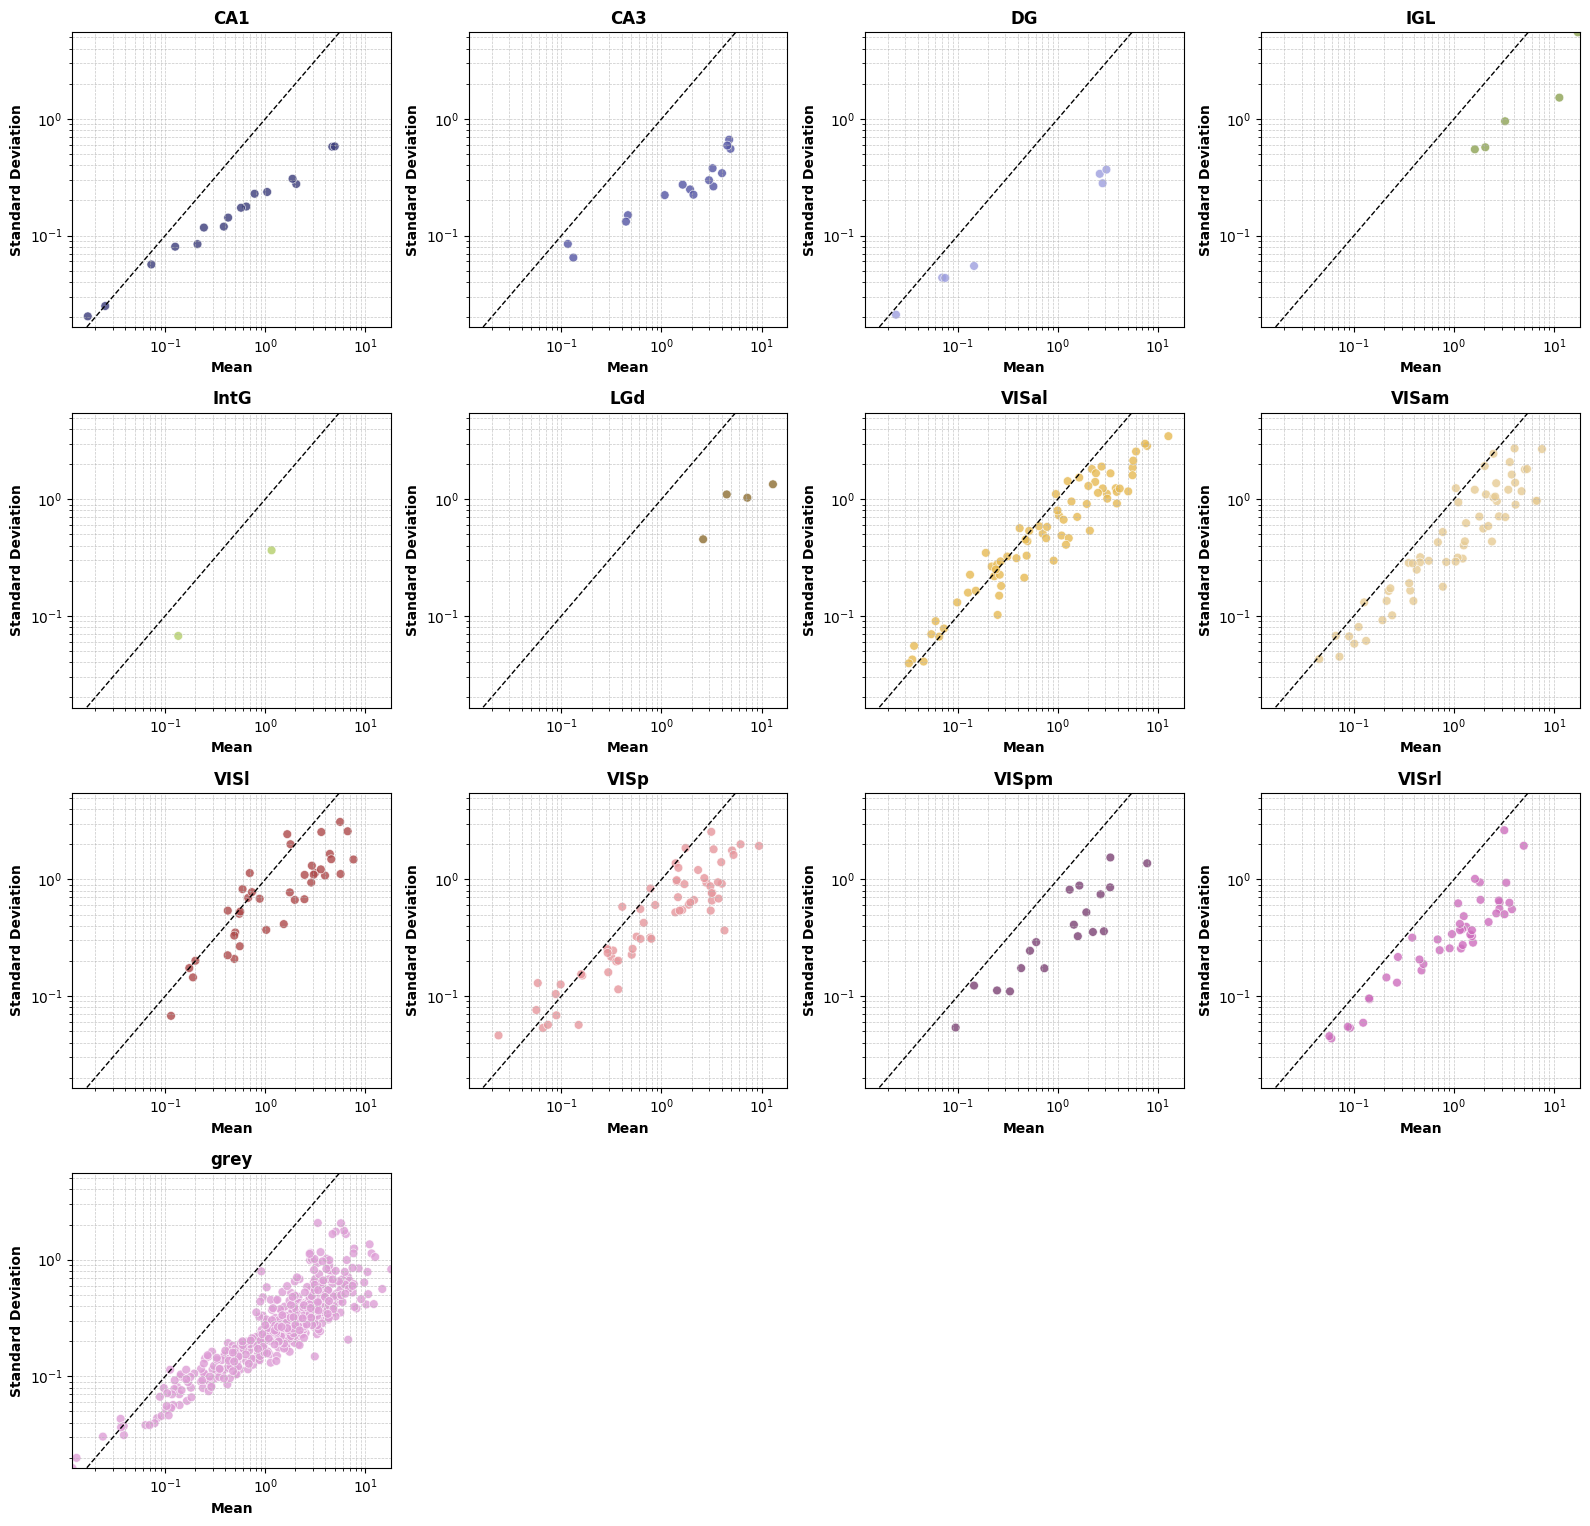
\includegraphics[width=\linewidth]{report_images/unit_firing_rate_statistics_single.png}
\caption{Individual firing rate statistics for each brain region.}
\label{fig:firing_rate_single}
\end{figure}

\begin{figure}[ht]
\centering
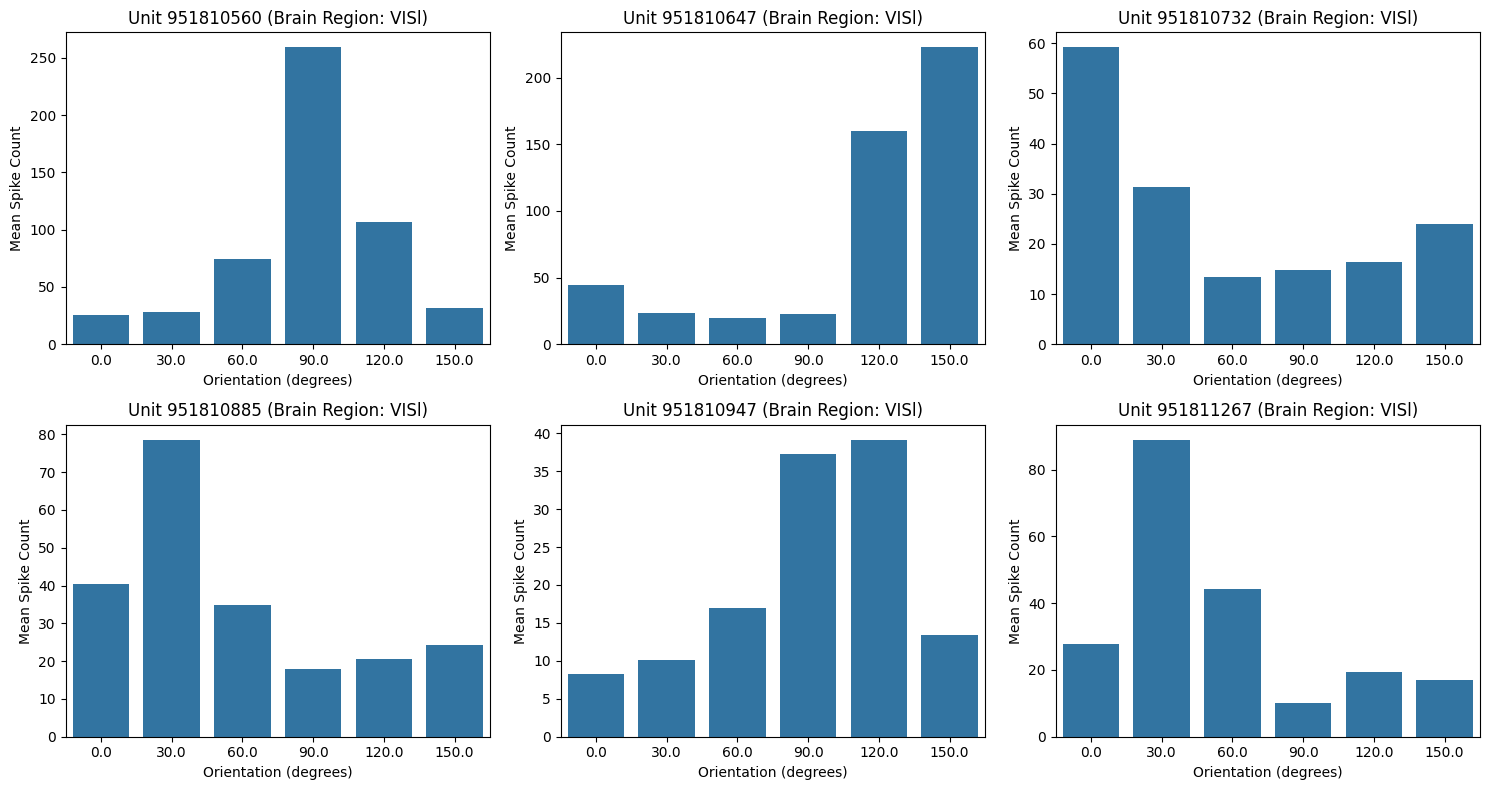
\includegraphics[width=\linewidth]{report_images/static_tuning_curves.png}
\caption{Tuning curves for static gratings.}
\label{fig:static_tuning}
\end{figure}

\begin{figure}[ht]
\centering
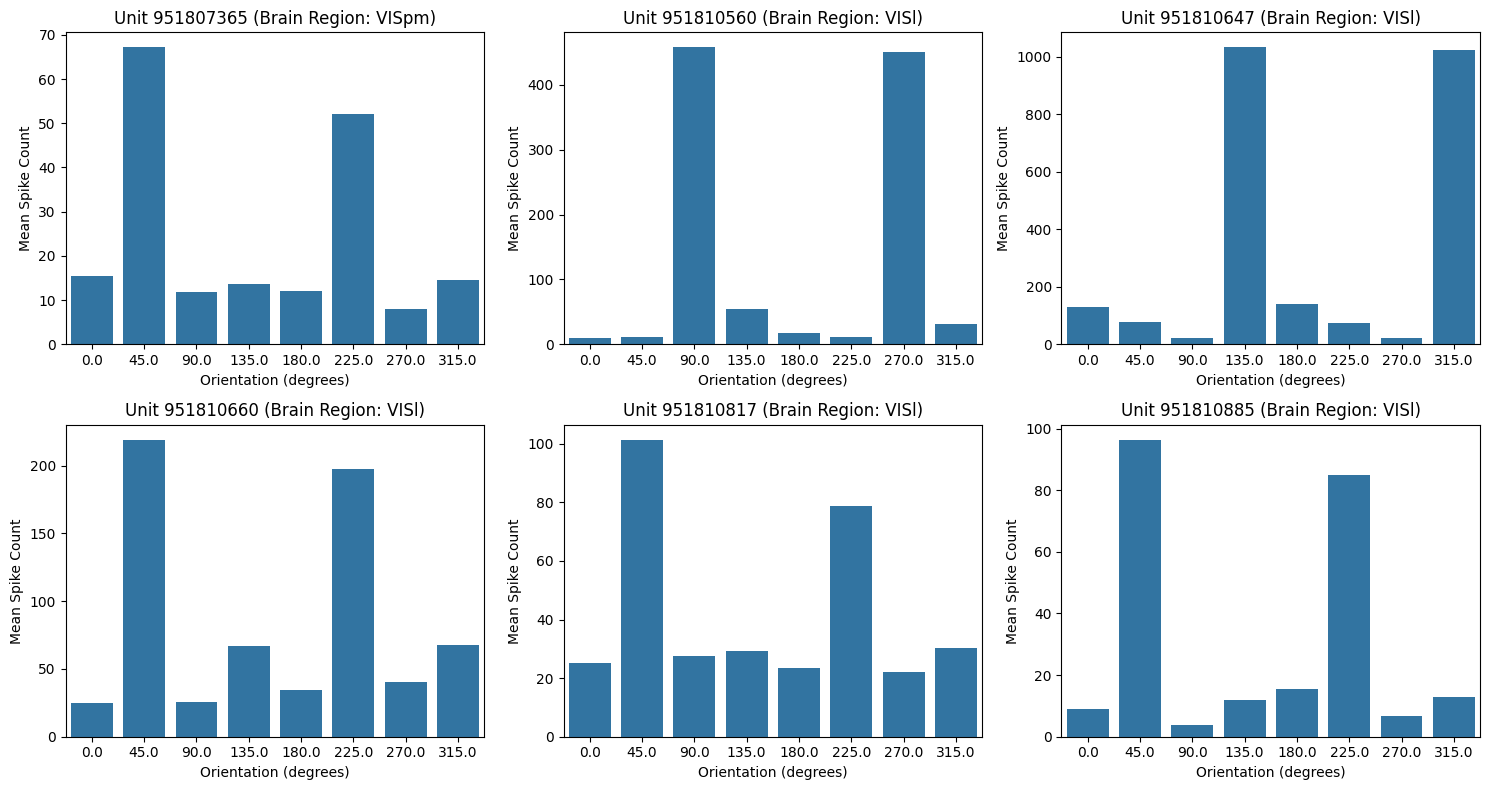
\includegraphics[width=\linewidth]{report_images/Drifting_tuning_curves.png}
\caption{Tuning curves for drifting gratings.}
\label{fig:drifting_tuning}
\end{figure}

\begin{figure}[ht]
\centering
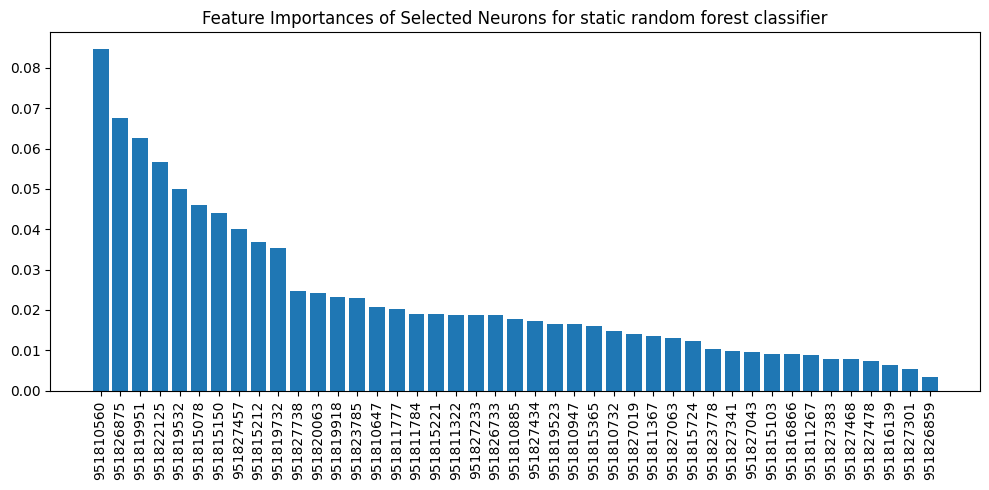
\includegraphics[width=\linewidth]{report_images/static_feature_selection.png}
\caption{Feature selection for static gratings.}
\label{fig:static_feature}
\end{figure}

\begin{figure}[ht]
\centering
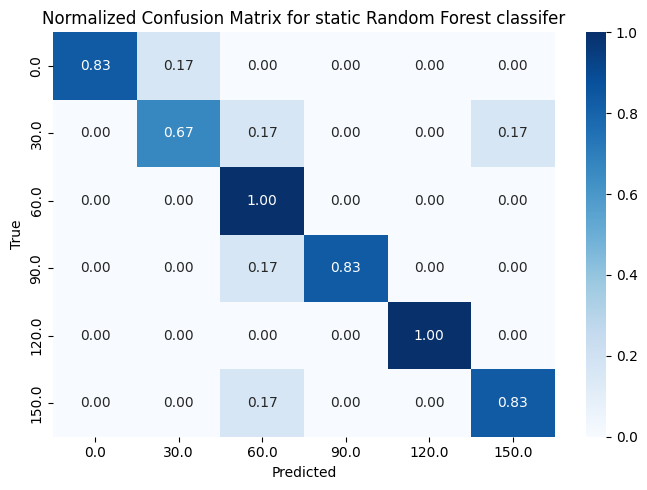
\includegraphics[width=\linewidth]{report_images/static_random_forest_confusion_matrix.png}
\caption{Random Forest confusion matrix for static gratings.}
\label{fig:static_rf_cm}
\end{figure}

\begin{figure}[ht]
\centering
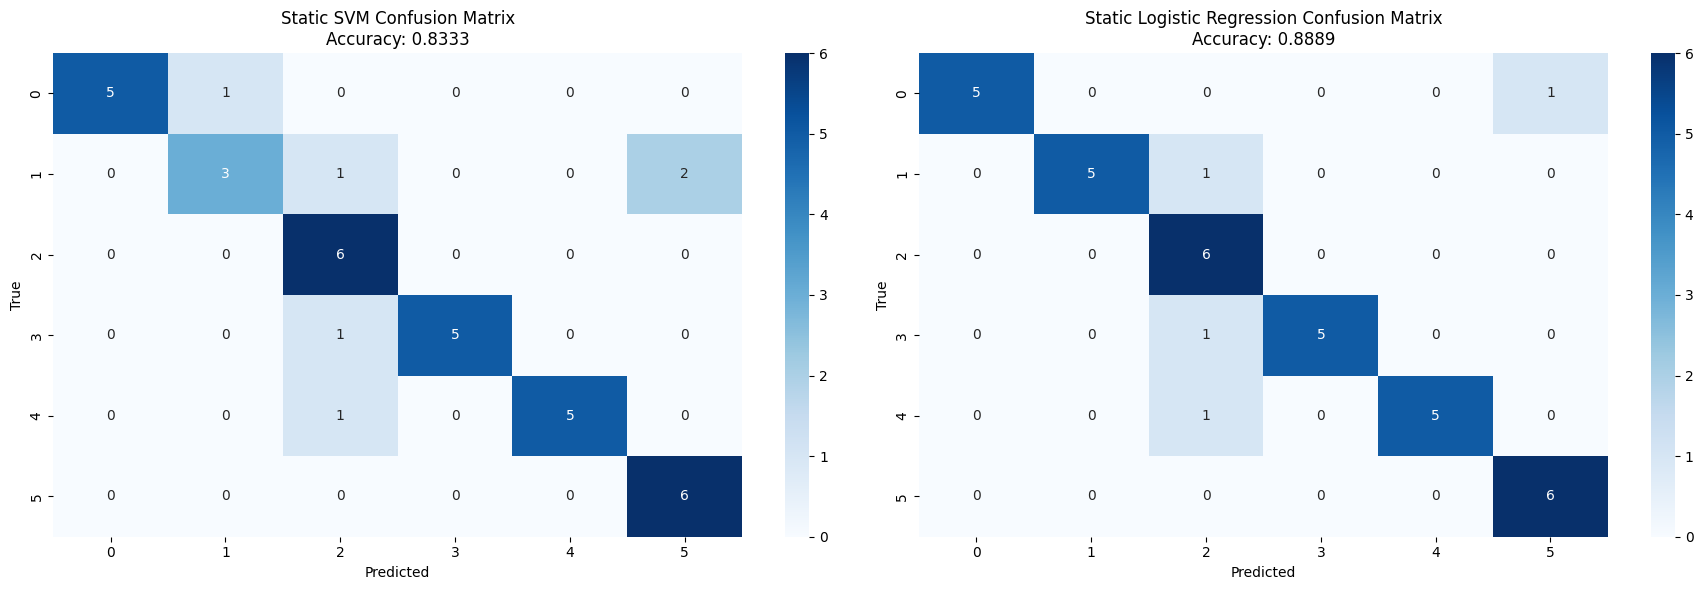
\includegraphics[width=\linewidth]{report_images/static_SVM_LogR_confusion_matrix.png}
\caption{SVM and Logistic Regression confusion matrices for static gratings.}
\label{fig:static_svm_logr_cm}
\end{figure}

\begin{figure}[ht]
\centering
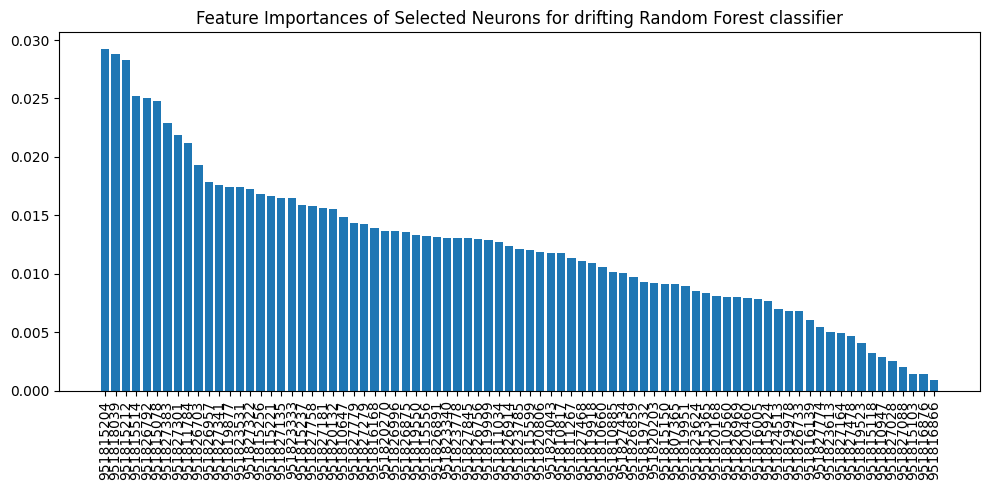
\includegraphics[width=\linewidth]{report_images/drifting_feature_selection.png}
\caption{Feature selection for drifting gratings.}
\label{fig:drifting_feature}
\end{figure}

\begin{figure}[ht]
\centering
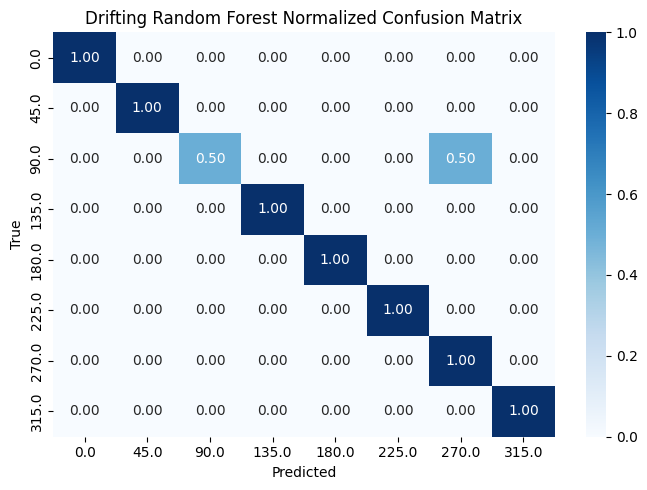
\includegraphics[width=\linewidth]{report_images/drifting_random_forest_confusion_matrix.png}
\caption{Random Forest confusion matrix for drifting gratings.}
\label{fig:drifting_rf_cm}
\end{figure}

\begin{figure}[ht]
\centering
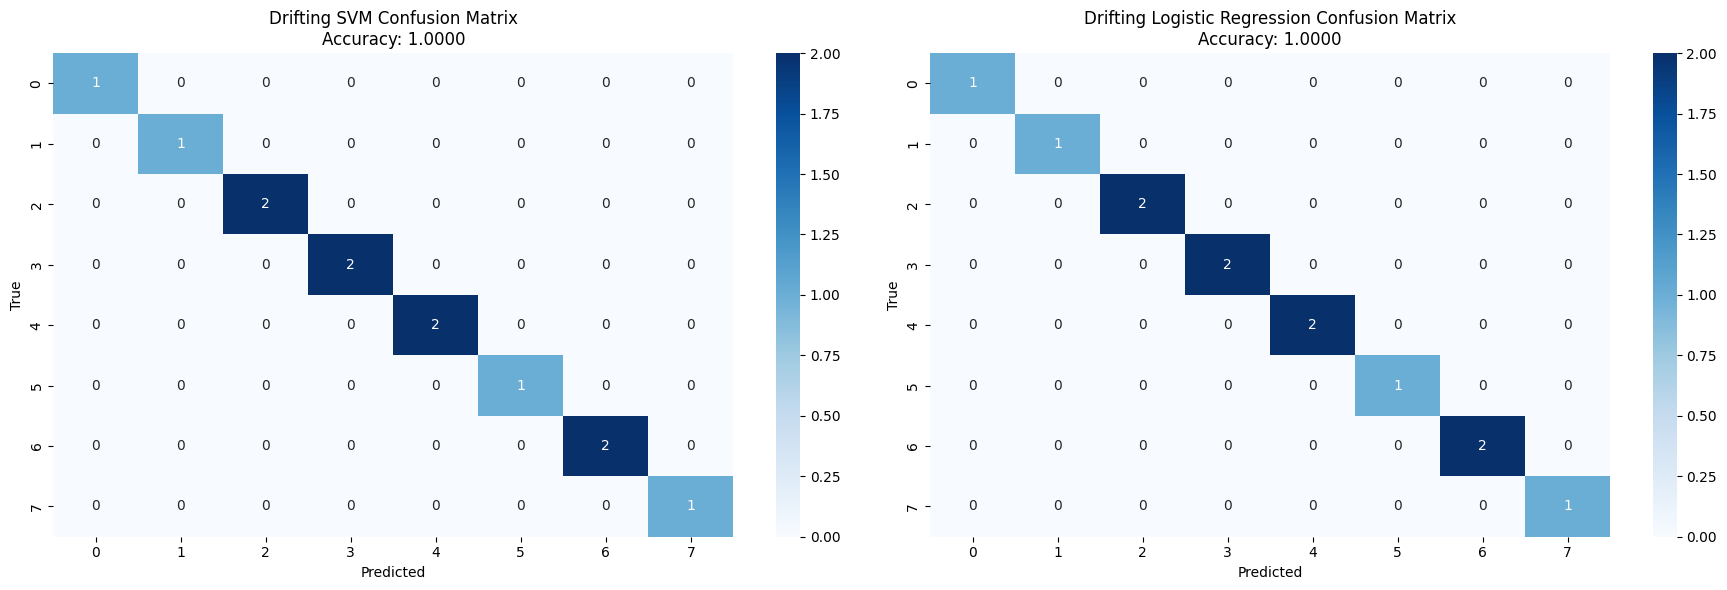
\includegraphics[width=\linewidth]{report_images/drifting_SVM_LogR_confusion_matrix.png}
\caption{SVM and Logistic Regression confusion matrices for drifting gratings.}
\label{fig:drifting_svm_logr_cm}
\end{figure}

\begin{figure}[ht]
\centering
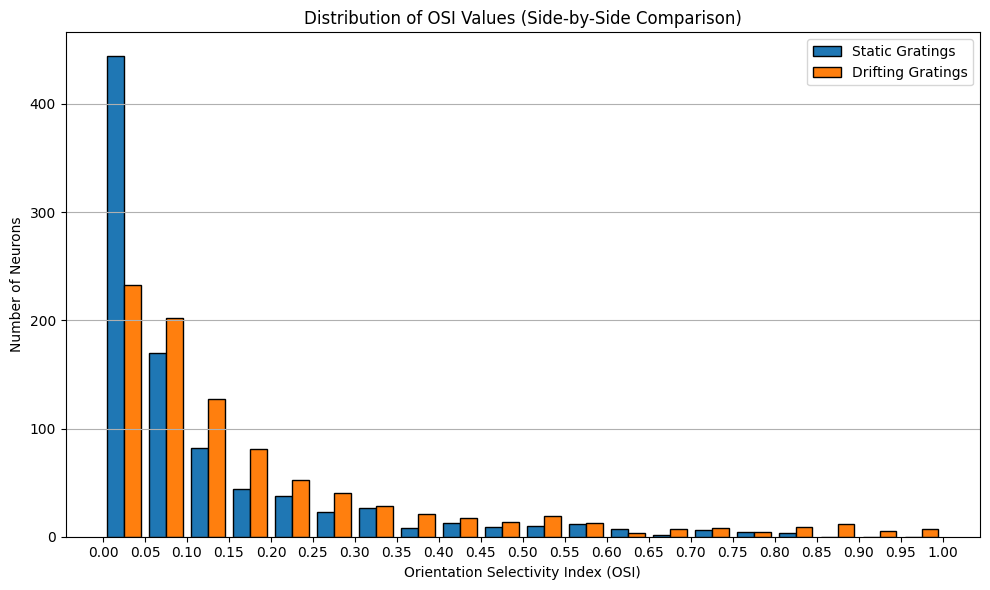
\includegraphics[width=\linewidth]{report_images/tuning_curves_comparison.png}
\caption{Comparison of tuning curves between static and drifting gratings.}
\label{fig:tuning_comparison}
\end{figure}

\begin{figure}[ht]
\centering
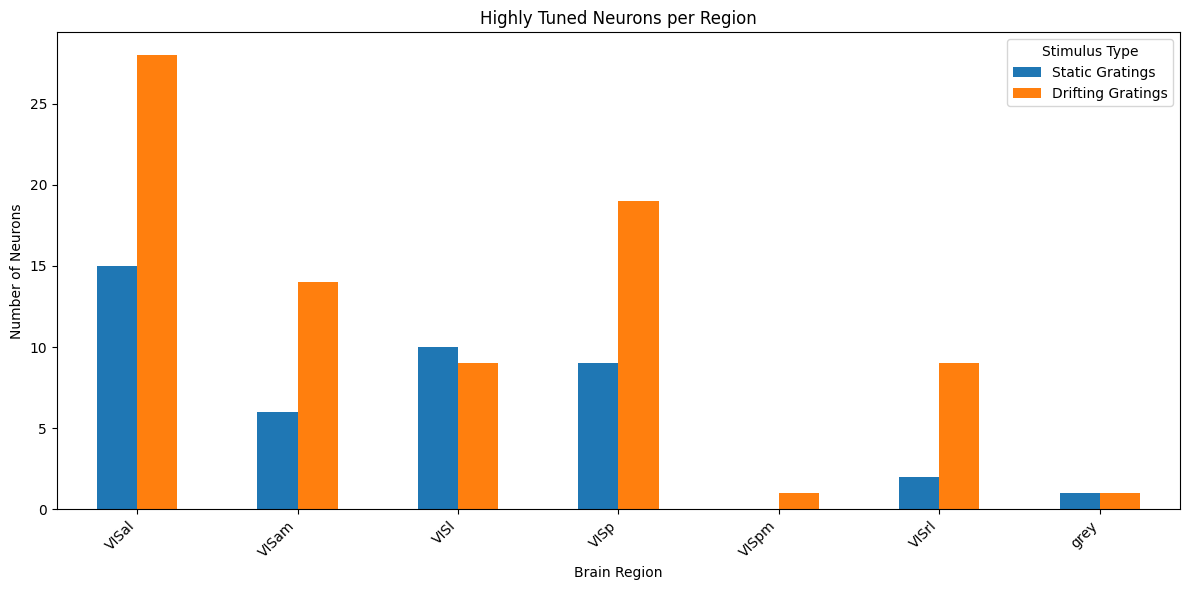
\includegraphics[width=\linewidth]{report_images/tuned_neurons_region.png}
\caption{Distribution of orientation-selective neurons across brain regions.}
\label{fig:tuned_regions}
\end{figure}

\end{document}